\chapter{The Initial Mass Function: Observations}
\label{ch:imf_obs}

\marginnote{
\textbf{Suggested background reading:}
\begin{itemize}
\item \href{http://adsabs.harvard.edu/abs/2014prpl.conf...53O}{Offner, S.~S.~R., et al. 2014, in ``Protostars and Planets VI", ed.~H.~Beuther et al., pp.~53-75} \nocite{offner14a}
\end{itemize}
\textbf{Suggested literature:}
\begin{itemize}
\item \href{http://adsabs.harvard.edu/abs/2010Natur.468..940V}{van Dokkum, P.~G., \& Conroy, C. 2010, Nature, 468, 940} \nocite{van-dokkum10a}
\item \href{http://adsabs.harvard.edu/abs/2012ApJ...748...14D}{da Rio, N., et al. 2012, ApJ, 748, 14} \nocite{da-rio12a}
\end{itemize}
}


As we continue to march downward in size scale, we now turn from the way gas clouds break up into clusters to the way clusters break up into individual stars. This is the subject of the initial mass function (IMF), the distribution of stellar masses at formation. The IMF is perhaps the single most important distribution in stellar and galactic astrophysics. Almost all inferences that go from light to physical properties for unresolved stellar populations rely on an assumed form of the IMF, as do almost all models of galaxy formation and the ISM.

\section{Resolved Stellar Populations}

There are two major strategies for determining the IMF from observations. One is to use direct star counts in regions where we can resolve individual stars. The other is to use integrated light from more distant regions where we cannot.

\subsection{Field Stars}

The first attempts to measure the IMF were by \citet{salpeter55a},\footnote{This has to be one of the most cited papers in all of astrophysics -- nearly 5,000 citations as of this writing.} using stars in the Solar neighborhood, and the use of Solar neighborhood stars remains one of the main strategies for measuring the IMF today. Suppose that we want to measure the IMF of the field stars within some volume or angular region around the Sun. What steps must we carry out? 

\paragraph{Constructing the Luminosity Function}

The first step is to construct a luminosity function for the stars in our survey volume in one or more photometric bands. This by itself is a non-trivial task, because we require absolute luminosities, which means we require distances. If we are carrying out a volume-limited instead of a flux-limited survey, we also require distances to determine if the target stars are within our survey volume.

The most accurate distances available are from parallax, but this presents a challenge. To measure the IMF, we require a sample of stars that extends down to the lowest masses we wish to measure. As one proceeds to lower masses, the stars very rapidly become dimmer, and as they become dimmer it becomes harder and harder to obtain accurate parallax distances. For $\sim 0.1$ $M_\odot$ stars, typical absolute V band magnitudes are $M_V \sim 14$, and parallax catalogs at such magnitudes are only complete out to $\sim 5-10$ pc. A survey of this volume only contains $\sim 200-300$ stars and brown dwarfs, and this sample size presents a fundamental limit on how well the IMF can be measured. If one reduces the mass range being studied, parallax catalogs can go out somewhat further, but then one is trading off sample size against the mass range that the study can probe. Hopefully \textit{Gaia} will improve this situation significantly.

\begin{marginfigure}
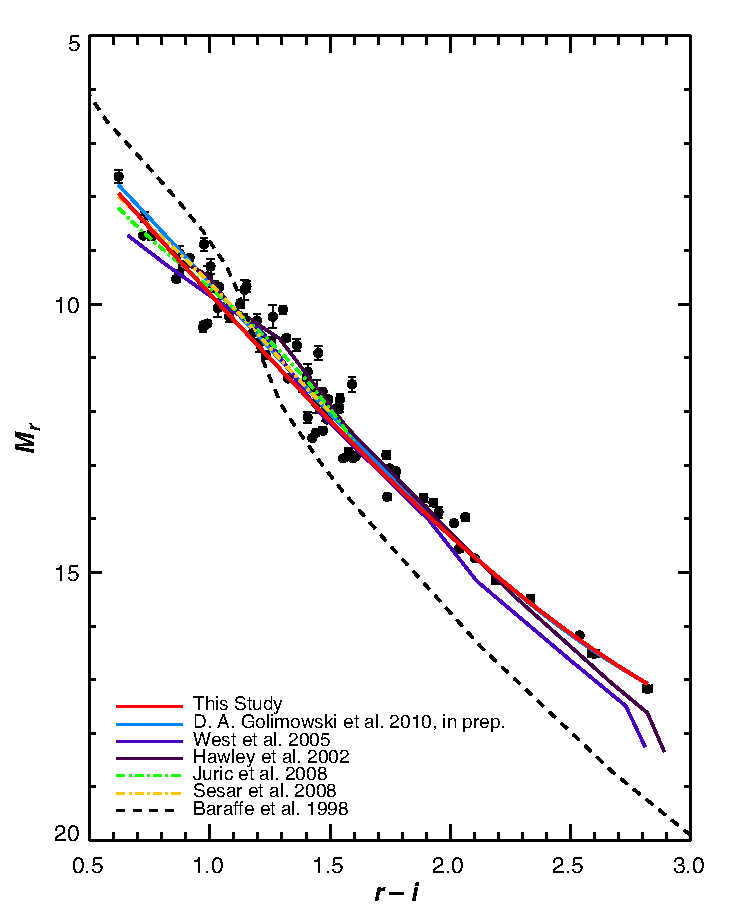
\includegraphics[width=\linewidth]{cmd_bochanski10}
\caption[Color-magnitude diagram of nearby stars]{
\label{fig:cmd_bochanski10}
Color-magnitude diagram for stars with well-measured parallax distances. The filters used are the SDSS $r$ and $i$. Credit: \citet{bochanski10a}, \copyright AAS. Reproduced with permission.
}
\end{marginfigure}

For these reasons, more recent studies have tended to rely on less accurate spectroscopic or photometric distances. These introduce significant uncertainties in the luminosity function, but they are more than compensated for by the vastly larger number of stars available, which in the most recent studies can be $>10^6$. The general procedure for photometric distances is to construct color-magnitude (CMD) diagrams in one or more colors for Solar neighborhood stars using the limited sample of stars with measured parallax distances, perhaps aided by theoretical models. Figure \ref{fig:cmd_bochanski10} shows an example of such a CMD. Each observed star with an unknown distance is then assigned an absolute magnitude based on its color and the CMD. The absolute magnitude plus the observed magnitude also gives a distance. The spectroscopic parallax method is analogous, except that one uses spectral type - magnitude diagrams (STMD) in place of color-magnitude ones to assign absolute magnitudes. This can be more accurate, but requires at least low resolution spectroscopy instead of simply photometry.

\paragraph{Bias Correction}

Once that procedure is done, one has in hand an absolute luminosity function, either over a defined volume or (more-commonly) a defined absolute magnitude limit. The next step is to correct it for a series of biases. We will not go into the technical details of how the corrections are made, but it is worth going through the list just to understand the issues, and why this is not a trivial task.

\textit{Metallicity bias:} the reference CMDs or STMDs used to assign absolute magnitudes are constructed from samples very close to the Sun with parallax distances. However, there is a known negative metallicity gradient with height above the galactic plane, so a survey going out to larger distances will have a lower average metallicity than the reference sample. This matters because stars with lower metallicity have higher effective temperature and earlier spectral type than stars of the same mass with lower metallicity. (They have slightly higher absolute luminosity as well, but this is a smaller effect.) As a result, if the CMD or spectral type-magnitude diagram used to assign absolute magnitudes is constructed for Solar metallicity stars, but the star being observed is sub-Solar, then we will tend to assign too high an absolute luminosity based on the color, and, when comparing with the observed luminosity, too large a distance. We can correct for this bias if we know the vertical metallicity gradient of the galaxy.

\textit{Extinction bias:} the reference CMDs / STMDs are constructed for nearby stars, which are systematically less extincted than more distant stars because their light travels through less of the dusty Galactic disk. Dust extinction reddens starlight, which causes the more distant stars to be assigned artificially red colors, and thus artificially low magnitudes. This in turn causes their absolute magnitudes and distances to be underestimated, moving stars from their true luminosities to lower values. These effects can be mitigated with knowledge of the shape of the dust extinction curve and estimates of how much extinction there is likely to be as a function of distance.

\textit{Malmquist bias:} there is some scatter in the magnitudes of stars at fixed color, both due to the intrinsic physical width of the main sequence (e.g., due to varying metallicity, age, stellar rotation) and due to measurement error. Thus at fixed color, magnitudes can scatter up or down. Consider how this affects stars that are near the distance of magnitude limit for the survey: stars whose true magnitude should place them just outside the survey volume or flux limit will be artificially scatter into the survey if they scatter up but not if they scatter down, and those whose true magnitude should place them within the survey will be removed if they scatter to lower magnitude. This asymmetry means that, for stars near the distance or magnitude cutoff of the survey, the errors are not symmetric; they are much more likely to be in the direction of positive than negative flux. This effect is known as Malmquist bias. It can be corrected to the extent that one has a good idea of the size of the scatter in magnitude and understands the survey selection.

\textit{Binarity:} many stars are members of binary systems, and all but the most distant of these will be unresolved in the observations and will be mistaken for a single star. This has a number of subtle effects, which we can think of in two limiting cases. If the binary is far from equal mass, say $q = M_2/M_1 \sim 0.3$ or less, then the secondary star contributes little light, and the system colors and absolute magnitude will not be that different from those of an isolated primary of the same mass. Thus the main effect is that we correctly include the primary in our survey, but we miss the secondary entirely, and therefore undercount the number of low luminosity stars. On the other hand, if the mass ratio $q\sim 1$, then the main effect is that the color stays about the same, but using our CMD we assign the luminosity of a single star when the true luminosity is actually twice that. We therefore underestimate the distance, and artificially scatter things into the survey (if it is volume limited) or out of the survey (if it is luminosity-limited). At intermediate mass ratios, we get a little of both effects.

The main means of correcting for this is, if we have a reasonable estimate of the binary fraction and mass ratio distribution, to guess a true luminosity function, determine which stars are binaries, add them together as they would be added in the observation, filter the resulting catalog through the survey selection, and compare to the observed luminosity function. This procedure is then repeated, adjusting the guessed luminosity function, until the simulated observed luminosity function matches the actually observed one. 

\begin{marginfigure}
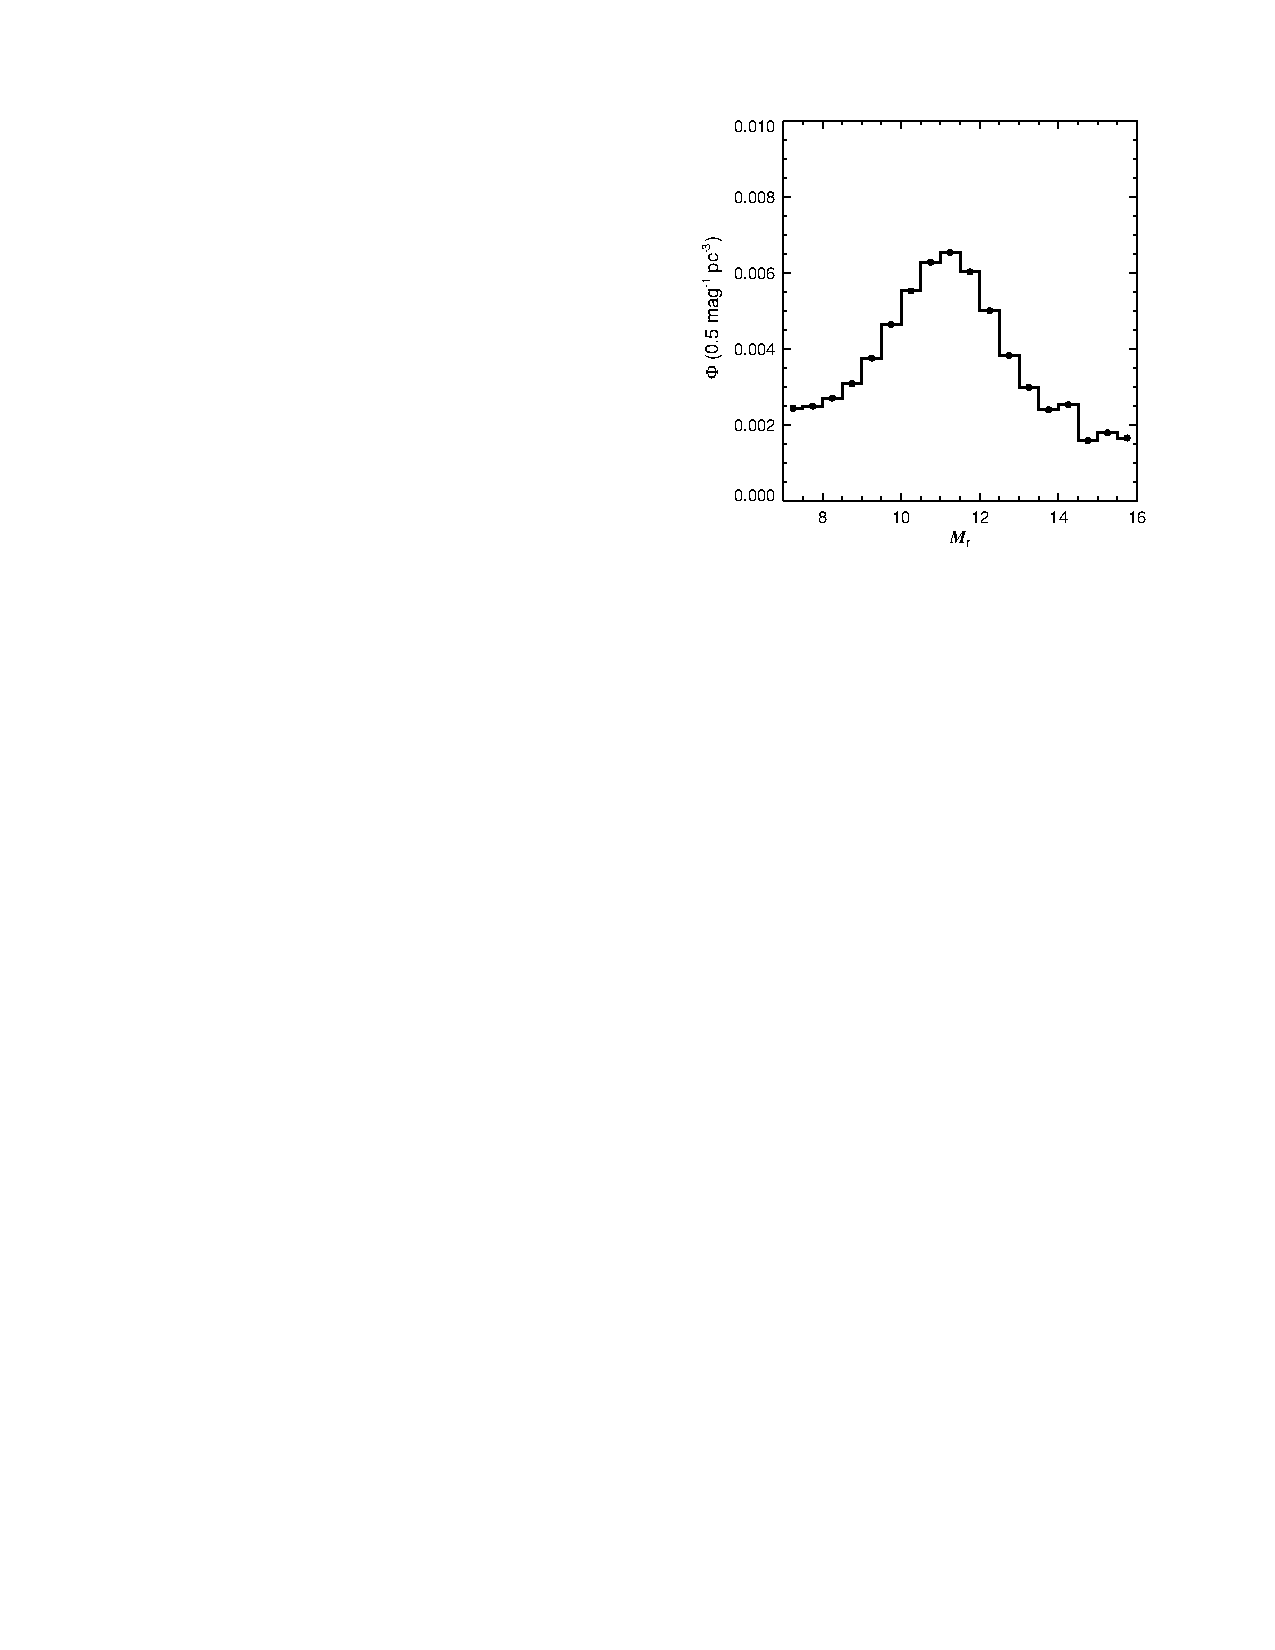
\includegraphics[width=\linewidth]{lumfunction_bochanski10}
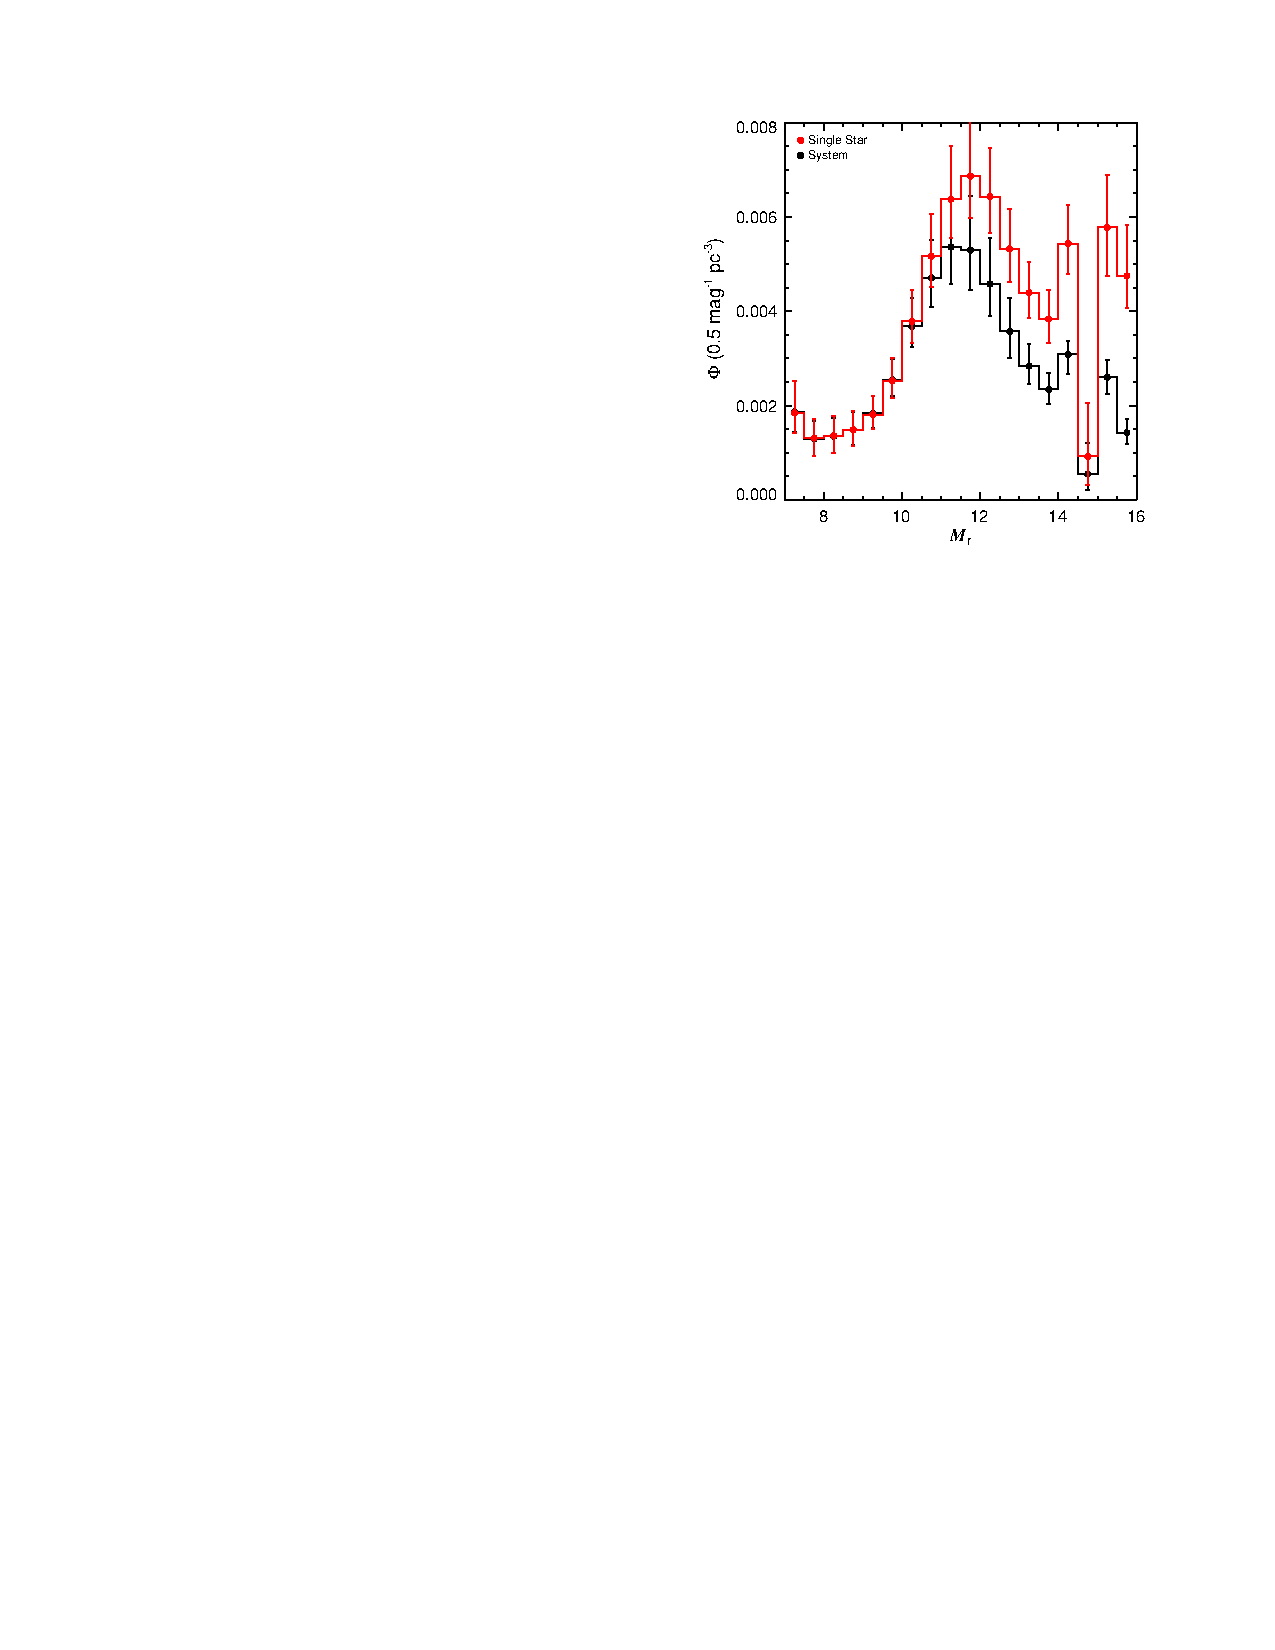
\includegraphics[width=\linewidth]{lumfunction_corr_bochanski10}
\caption[Color-magnitude diagram of nearby stars]{
\label{fig:lumfunction_bochanski10}
Luminosity function for Milky Way stars before (top) and after (bottom) bias correction. Credit: \citet{bochanski10a}, \copyright AAS. Reproduced with permission.
}
\end{marginfigure}

Once all these bias corrections are made, the result is a corrected luminosity function that (should) faithfully reproduce the actual luminosity function in the survey volume. Figure \ref{fig:lumfunction_bochanski10} shows an example of raw and corrected luminosity functions.


\paragraph{The Mass-Magnitude Relation}

The next step is to convert the luminosity function into a mass function, which requires knowledge of the mass-magnitude relation (MMR) in whatever photometric band we have used for our luminosity function. This must be determined by either theoretical modelling, empirical calibration, or both. Particularly at the low mass end, the theoretical models tend to have significant uncertainties arising from complex atmospheric chemistry that affects the optical and even near-infrared colors. 
For empirical calibrations, the data are only as good as the empirical mass determinations, which must come from orbit modelling. This requires the usual schemes for measuring stellar masses from orbits, e.g., binaries that are both spectroscopic and eclipsing and thus have known inclinations, or visual binaries with measured radial velocities. Figure \ref{fig:mmr_delfosse00} shows an example empirical MMR.

\begin{marginfigure}
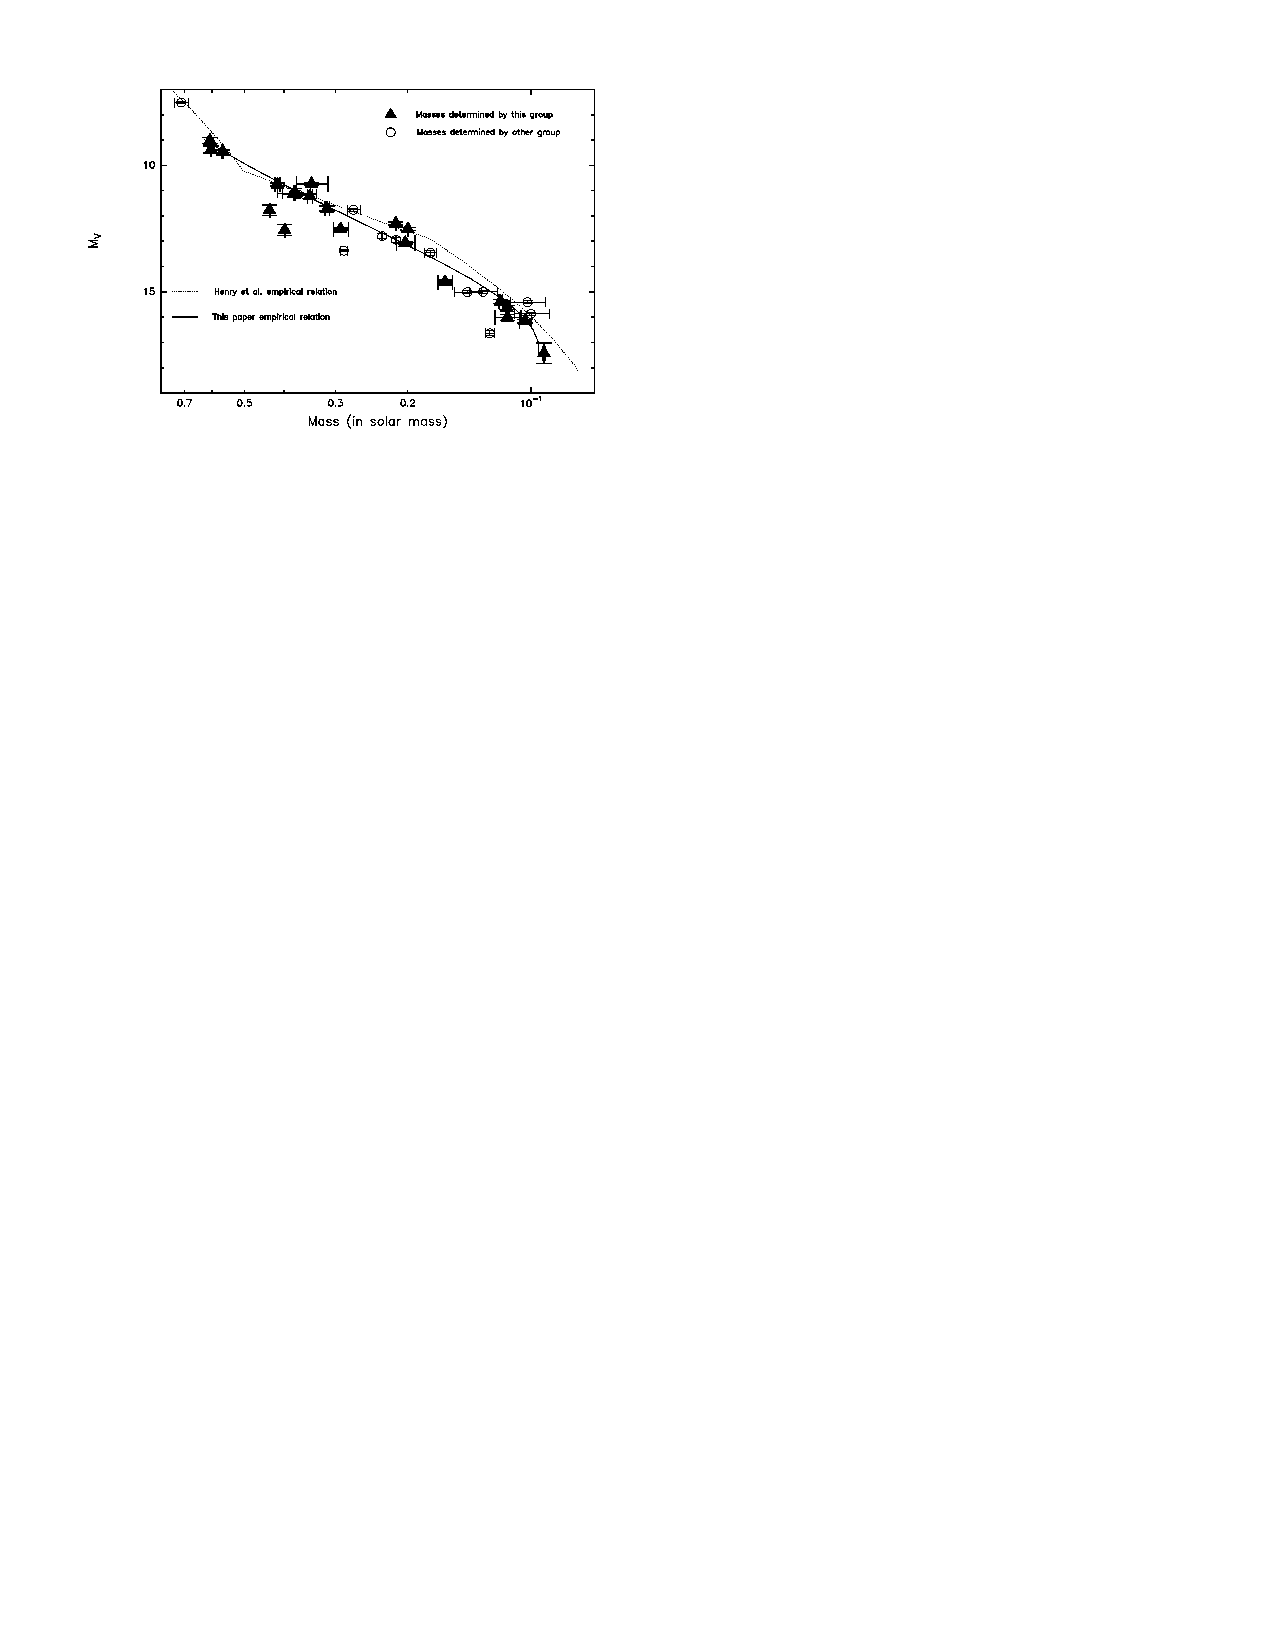
\includegraphics[width=\linewidth]{mmr_delfosse00}
\caption[Mass-magnitude relationship]{
\label{fig:mmr_delfosse00}
Empirically-measured mass-magnitude relationship in $V$ band. Credit: \citeauthor{delfosse00a}, A\&A, 364, 217, 2000, reproduced with permission \copyright\, ESO.
}
\end{marginfigure}

As with the luminosity function, there are a number of possible biases, because the stars are not uniform in either age or metallicity, and as a result there is no true single MMR. This would only introduce a random error if the age and metallicity distribution of the sample used to construct the MMR were the same as that in the IMF survey. However, there is no reason to believe that this is actually the case. The selection function used to determine the empirical mass-magnitude sample is complex and poorly characterized, but it is certainly biased towards systems closer to the Sun, for example. Strategies to mitigate this are similar to those used to mitigate the corresponding biases in the luminosity function.

Once the mass-magnitude relationship and any bias corrections have been applied, the result is a measure of the field IMF. The results appear to be well-fit by a lognormal distribution or a broken powerlaw, along the lines of the \citet{chabrier05a} and \citet{kroupa02c} IMFs introduced in Chapter \ref{ch:obsstars}.

\paragraph{Age Correction}

The strategy we have just described works fine for stars up to $\sim 0.7$ $M_\odot$ in mass. However, it fails with higher mass stars, for one obvious reason: stars with masses larger than this can evolve off the main sequence on timescales comparable to the mean stellar age in the Solar neighborhood. Thus the quantity we measure from this procedure is the present-day mass function (PDMF), not the IMF. Even that is somewhat complicated because stars' luminosities start to evolve non-negligibly even before they leave the main sequence, so there are potential errors in assigning masses based on a MMR calibrated from younger stars.

One option in this case is simply to give up and not say anything about the IMF at higher masses. However, there is another option, which is to try to correct for the bias introduced by stellar evolution. Suppose that we think we know both the star formation history of the region we are sampling, $\dot{M}_*(t)$, and the initial mass-dependent main-sequence stellar lifetime, $t_{\rm MS}(m)$. Let $dn/dm$ be the IMF. In this case, the total number of stars formed of the full lifetime of the galaxy in a mass bin from $m$ to $m+dm$ is
\begin{equation}
\frac{dn_{\rm form}}{dm} =  \frac{dn}{dm} \int_{-\infty}^0 dt \, \dot{M}_*(t)
\end{equation}
where $t=0$ represents the present. In contrast, the number of stars per unit mass still on the main sequence is
\begin{equation}
\frac{dn_{\rm MS}}{dm} = \frac{dn}{dm} \int_{-t_{\rm MS}(m)}^0 dt \, \dot{M}_*(t)
\end{equation}
Thus if we measure the main sequence mass distribution $dn_{\rm MS}/dm$, we can correct it to the IMF just by multiplying:
\begin{equation}
\frac{dn}{dm} \propto \frac{dn_{\rm MS}}{dm} \frac{\int_{-t_{\rm MS}(m)}^0 dt \, \dot{M}_*(t)}{\int_{-\infty}^0 dt \, \dot{M}_*(t)}.
\end{equation}
This simply reduces to scaling the number of observed stars by the fraction of stars in that mass bin that are still alive today.

Obviously this correction is only as good as our knowledge of the star formation history, and it becomes increasingly uncertain as the correction factor becomes larger. Thus attempts to measure the IMF from the Galactic field even with age correction are generally limited to masses of no more than a few $M_\odot$.

\subsection{Young Clusters}

To measure the IMF for more massive stars requires a different technique: surveys of young star clusters. The overall outline of the technique is essentially the same as for the field: construct a luminosity function, correct for biases, then use a mass-magnitude relation to convert to a mass function. However, compared to the field, studying a single cluster offers numerous advantages:
\begin{itemize}
\item If the population is young enough, then even the most massive stars will remain on the main sequence, so there is no need to worry about correcting from the PDMF to the IMF. Even for somewhat older clusters, one can probe to higher masses than would be possible with the $\sim 5-10$ Gyr old field population.
\item The stellar population is generally uniform in metallicity or very close to it, so there are no metallicity biases.
\item The entire stellar population is at roughly the same distance, so there are no Malmquist or extinction biases. Moreover, in some cases the distance to the cluster is known to better than 10\% from radio parallax -- some young stars flare in the radio, and with radio interferometry it is possible to obtain parallax measurements at much larger distances than would be possible for the same stars in the optical. 
\item Low-mass stars and brown dwarfs are significantly more luminous at young ages, and so the same magnitude limit will correspond to a much lower mass limit, making it much easier to probe into the brown dwarf regime.
\end{itemize}

These advantages also come with some significant costs.
\begin{itemize}
\item The statistics are generally much worse than for the field. The most populous young cluster that is close enough for us to resolve individual stars down to the hydrogen burning limit is the Orion Nebula Cluster, and it contains only $\sim 10^3 - 10^4$ stars, as compared to $\sim 10^6$ for the largest field surveys.
\item The MMR that is required to convert an observed magnitude into a mass is much more complex in a young cluster, because a significant fraction of the stars may be pre-main sequence. For such stars, the magnitude is a function not just of the mass but also the age, and one must fit both simultaneously, and with significant theoretical uncertainty. We will discuss this issue further in Chapter \ref{ch:protostar_evol}. How much of a problem this is depends on the cluster age -- for a 100 Myr-old cluster like the Pleiades, all the stars have reached the main sequence, while for a $\sim 1-2$ Myr-old cluster like Orion, almost none have. However, there is an obvious tradeoff here: in a Pleiades-aged cluster, the correction for stars leaving the main sequence is significant, while for an Orion-aged cluster it is negligible.
\item For the youngest clusters, there is usually significant dust in the vicinity of the stars, which introduces extinction and reddening that is not the same from star to star. This introduces scatter, and also potentially bias because the extinction may vary with position, and there is a systematic correlation between position and mass (see next point).
\item Mass segregation can be a problem. In young clusters, the most massive stars are generally found closer to the center -- whether this is a result of primordial mass segregation (the stars formed there) or dynamical mass segregation (they formed elsewhere but sank to the center), the result is the same. Conversely, low mass stars are preferentially on the cluster outskirts. This means that studies must be extremely careful to measure the IMF over the full cluster, not just its outskirts or core; this can be hard in the cluster center due to problems with crowding. Moreover, if the extinction is not spatially uniform, more massive stars toward the cluster center are likely to suffer systematically more extinction that low-mass ones.
\item Dynamical effects can also be a problem. A non-trivial fraction of O and B stars are observed to be moving with very high spatial velocities, above $\sim 50$ km s$^{-1}$. These are known as runaways. They are likely created by close encounters between massive stars in the core of a newly-formed cluster that lead to some stars being ejected at speeds comparable to the orbital velocities in the encounter. Regardless of the cause, the fact that this happens means that, depending on its age and how many ejections occurred, the cluster may be missing some of its massive stars. Conversely, because low-mass stars are further from the center, if there is any tidal stripping, that will preferentially remove low-mass stars.
\item Binary correction is harder for young stars because the binary fraction as a function of mass is much less well known for young clusters than it is for field stars.
\end{itemize}

Probably the best case for studying a very young cluster is the Orion Nebula Cluster, which is 415 pc from the Sun. Its distance is known to a few percent from radio interferometry \citep{sandstrom07a, menten07a, kim08a}. It contains several thousand stars, providing relatively good statistics, and it is young enough that all the stars are still on the main sequence. It is close enough that we can resolve all the stars down to the brown dwarf limit, and even beyond. However, the ONC's most massive star is only 38 $M_\odot$, so to study the IMF at even higher masses requires the use of more distant clusters within which we cannot resolve down to low masses. 

For somewhat older clusters, the best case is almost certainly the Pleiades, which has an age of about 120 Myr. It obviously has no very massive stars left, but there are still $\sim 10$ $M_\odot$ stars present, and it is also close and very well-studied. The IMF inferred for the Pleiades appears to be consistent with that measured in the ONC.

\subsection{Globular Clusters}

A final method for studying the IMF is to look at globular clusters. Compared to young clusters, globular cluster lack the massive stars because they are old, and suffer somewhat more from confusion problems due to their larger distances. Otherwise they are quite similar in terms of methodological advantages and disadvantages.

The main reason for investigating globular clusters is that they provide us with the ability to measure the IMF in an environment as different as possible from that of young clusters forming in the disk of the Milky Way today. The stars in globular clusters are ancient and metal poor, and they provide the only means of accessing that population without resorting to integrated light measurements. They are therefore a crucial bridge to the integrated light methods we will discuss shortly.

The major challenge for globular clusters is that all the dynamical effects are much worse, due to the longer time that the clusters have had to evolve. Over long times, globular clusters systematically lose low-mass stars due to tidal shocking and a phenomenon known as two-body evaporation, whereby the cluster attempts to relax to a Maxwellian velocity distribution, but, due to the fact that the cluster is sitting in a tidal potential, the tail of that distribution keeps escaping. This alters the IMF. There can also be stellar collisions, which obviously move low mass stars into higher mass bins.

Accounting for all these effects is a major challenge, and the usual method is to adopt a proposed IMF and then try to simulate the effects of dynamical evolution over the past $\sim 13$ Gyr in order to predict the PDMF that would result. This is then compared to the observed PDMF, and the underlying IMF is iteratively adjusted until they match. This is obviously subject to considerable uncertainties.

\subsection{General Results}

The general result of these studies is that the IMF appears to be fairly universal. There are claims for variation in the literature, but they are generally based on statistical analyses that ignore (or underestimate) systematic errors, which are pervasive. This is not to say that the IMF certainly is universal, just that there is as yet no strongly convincing evidence for its variation. One possible exception is in the nuclear star cluster of the Milky Way, where \citet{lu13a} report an IMF that is somewhat flatter than usual at the high mass end. It is unclear if this is a true IMF effect resulting from the very strange formation environment, or a dynamical effect.


\section{Unresolved Stellar Populations}

The main limitation of studying the IMF using resolved stars is that it limits our studies to the Milky Way and, if we are willing to forgo observing below $\sim 1$ $M_\odot$, the Magellanic Clouds. This leaves us with a very limited range of star-forming environments to study, at least compared with the diversity of galaxies that has existed over cosmological time, or even that exist in the present-day Universe. To measure the IMF in more distant systems, we must resort to techniques that rely on integrated light from unresolved stars.

\subsection{Stellar Population Synthesis Methods}

One method for working with integrated light is stellar population synthesis: one starts with a proposed IMF, and then generates a prediction for the stellar light from it. In the case of star clusters or other mono-age populations, the predicted frequency-dependent luminosity from a stellar population of mass $M_*$ is
\begin{equation}
L_\nu = M_* \int_0^\infty dm \,\frac{dn}{dm} L_\nu(m,t),
\end{equation}
where $L_\nu(m,t)$ is the predicted specific luminosity of a star of mass $m$ and age $t$. For a population with a specified star formation history (usually constant), one must further integrate over the star formation history
\begin{equation}
L_\nu = \int_0^{\infty} dt\, \dot{M}_*(t) \int_0^\infty dm\, \frac{dn}{dm} L_\nu(m,t)
\end{equation}
where $\dot{M}_*(t)$ is the star formation rate a time $t$ in the past. The predicted spectrum can then be compared to observations to test whether the proposed IMF is consistent with them.

\paragraph{The Upper IMF} In practice when using this method to study the IMF, one selects combinations of photometric filters or particular spectral features that are particularly sensitive to certain regions of the IMF. One prominent example of this is the ratio of H$\alpha$ emission to emission in other bands (or to inferred total mass). This probes the IMF because H$\alpha$ emission is produced by recombinations, and thus the H$\alpha$ emission rate is proportional to the ionizing luminosity. This in turn is dominated by $\sim 50$ $M_\odot$ and larger stars. In contrast, other bands are more sensitive to lower masses -- how low depends on the choice of band, but even for the bluest non-ionizing colors (e.g., \textit{GALEX} FUV), at most $\sim 20$ $M_\odot$. Thus the ratio of H$\alpha$ to other types of emission serves as a diagnostic of the number of very massive stars per unit total mass or per unit lower mass stars, and thus of the shape of the upper end of the IMF.

When comparing models to observations using this technique, one must be careful to account for stochastic effects. Because very massive stars are rare, approximating the IMF using the integrals we have written down will produce the right averages, but the dispersion about this average may be very large and asymmetric. In this case Monte Carlo sampling of the IMF is required. Once one does that, the result is a predicted probability distribution of the ratio of H$\alpha$ to other tracers, or to total mass. One can then compare this to the observed distribution of luminosity ratio in a sample of star clusters in order to study whether those clusters' light is consistent with a proposed IMF. One can also use the same technique on entire galaxies (which are assumed to have constant star formation rates) in order to check if the integrated light from the galaxy is consistent with the proposed IMF.

This technique has been deployed in a range of nearby spirals and dwarfs, and the results are that, when the stochastic correction is properly included, the IMF is consistent with the same high end slope of roughly $dn/dm\propto m^{-2.3}$ seen in resolved star counts.

\paragraph{The Low-Mass IMF in Ellipticals} A second technique has been to target two spectral features that are sensitive to the low mass end of the IMF: the Na~\textsc{i} doublet and the Wing-Ford molecular FeH band. Both of these regions are useful because they are produced by absorption by species found only in M type stars, but they are also gravity-sensitive, so they are \textit{not} found in the spectra of M giants. They therefore filter out a contribution from red giants, and only include red dwarfs. The strength of these two features therefore measures the ratio of M dwarfs to K dwarfs, which is effectively the ratio of $\sim 0.1-0.3$ $M_\odot$ stars to $\sim 0.3-0.5$ $M_\odot$ stars.

\citet{van-dokkum10a} used this technique on stacked spectra of ellipticals in the Coma and Virgo clusters, and found that the spectral features there were \textit{not} consistent with the IMF seen in the Galactic field and in young clusters. Instead, they found that the spectrum required an IMF that continues to rise down to $\sim 0.1$ $M_\odot$ rather than having a turnover. This result was, and continues to be, highly controversial due to concerns about unforeseen systematics hiding in the stellar population synthesis modelling.

\begin{figure}
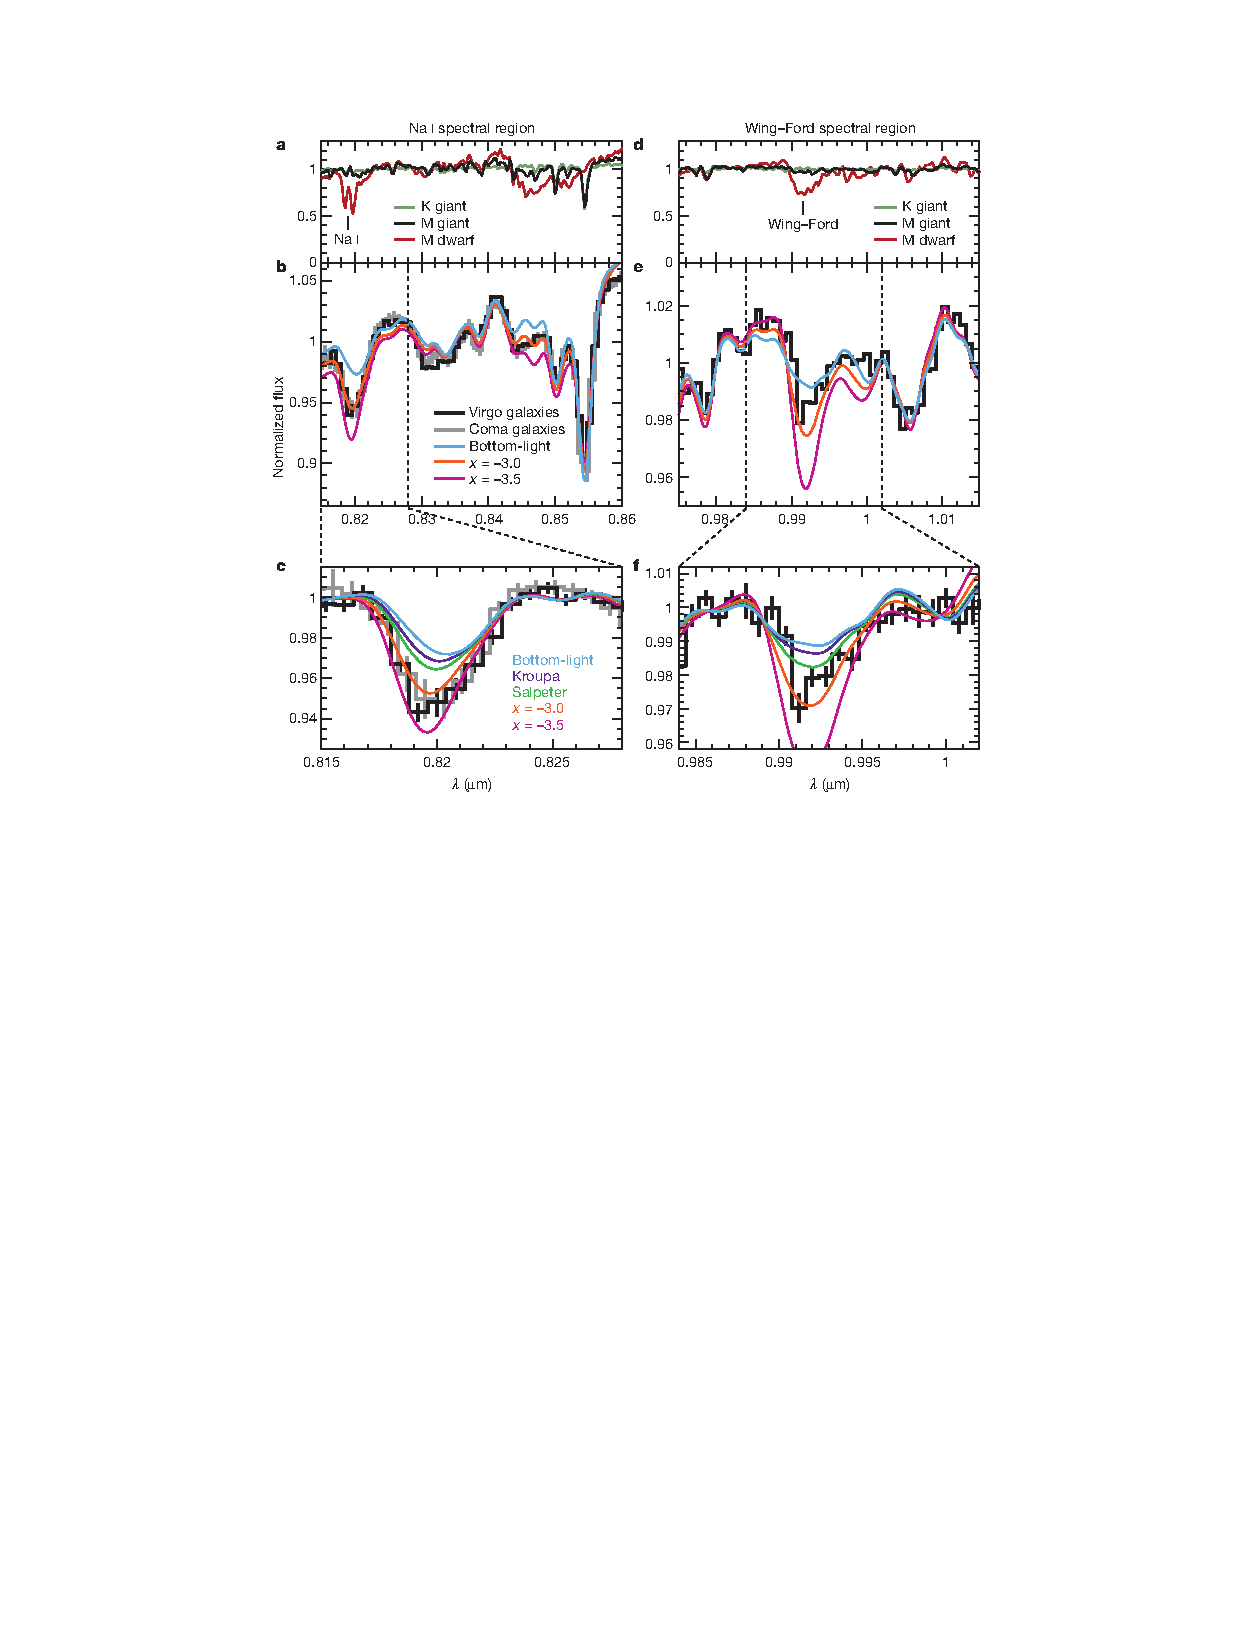
\includegraphics[width=\linewidth]{spectra_vdk10}
\caption[Elliptical galaxy spectra in the Na~\textsc{i} and Wing-Ford regions]{
\label{fig:spectra_vdk10}
Top panels: sample spectra of K and M giants and M dwarfs in the Na~\textsc{i} and Wing-Ford spectral regions. Middle panels: averaged spectra for Virgo cluster (black) and Coma cluster (gray) ellipticals, overlayed with predicted model spectra for four possible IMFs, ranging from "bottom light" (few dwarfs) to powerlaws of increasing steepness (more dwarfs). Bottom panels: zoom-ins on the Na~\textsc{i} and Wing-Ford regions in the previous panels. Taken from \citet{van-dokkum10a}.
}
\end{figure}

\subsection{Mass to Light Ratio Methods}

A second method of probing the IMF in unresolved stellar populations relies in measuring the mass independently of the starlight and thereby inferring a mass to light ratio that can be compared to models. As with the Na~\textsc{i} and Wing-Ford methods, this is most easily applied to old, gas-free stellar populations with no gas to complicate the modelling. One can obtain an independent measurement of the mass in two ways: from lensing of background objects, or from dynamical modelling in systems where the stellar velocity distribution as a function of position has been determined using an integrated field unit (IFU) or similar technique to get a spectrum at each position. Once it is obtained, the mass map is divided by the light map to form a mass to light ratio.

The main complication in comparing the mass to light ratio to theoretical predictions from stellar population synthesis is that one must account for dark matter, which can raise the ratio compared to that of a pure stellar system. This requires some modelling, and is probably the most uncertain part of the procedure. Of course if one allows a completely arbitrary distribution of dark matter, then one can produce any light to mass ratio that is heaver than one produced by the stars alone. However, this might require extremely implausible dark matter distributions. Thus the general procedure is to consider a set of "reasonable" dark matter distributions and infer limits on the stellar mass to light ratio from the extreme limiting cases.

A number of authors have used this technique \citep[e.g.,][]{cappellari12a} and tentatively found results consistent with those of \citet{van-dokkum10a}, i.e., that in giant elliptical galaxies the mass to light ratio is such that one must have an IMF that produces less light per unit mass than the Milky Way IMF.

\section{Binaries}

While this chapter is mostly about the IMF, the IMF is inextricably bound up with the properties of binary star systems. This is partly for observational reasons -- the need to correct observed luminosity functions for binarity -- and partly for theoretical reasons, which we will cover in Chapter \ref{ch:imf_th}. We will therefore close this chapter with a discussion of the observational status of the properties of binary stars, or stellar multiples more generally.

\subsection{Finding Binaries}

Before diving in, we will briefly review how we find stellar binaries. The history of this is interesting, because binary stars are one of the first examples of successful use of statistical inference in astronomy. Of course there are many stars that appear close together on the sky, but it is non-trivial to determine which are true companions and which are chance alignments. In the 1700s, it was not known if there were any true binary stars. However, in 1767 the British astronomer John Michell performed a statistical analysis of the locations of stars on the sky, and showed that there were more close pairs than would be expected from random placement. Here therefore concluded that there must be true binaries. What is particularly impressive is that this work predates a general understanding of Poisson distributions, which were not fully understood until Poisson's work in 1838.

Today binaries can be identified in several ways.
\begin{itemize}
\item {\it Spectroscopic binaries}: these are systems where the spectral lines of a star show periodic radial velocity variations that are consistent with the star moving in a Keplerian orbit. Single-lined spectroscopic binaries are those where only one star's moving lines are seen, and double-lined ones are systems where two sets of lines moving in opposite senses are seen. Spectroscopic detection is generally limited to binaries that are quite close, both for reasons of velocity sensitivity and for reasons of timescale -- wide orbits take too long to produce a noticeable change in radial velocity.
\item {\it Eclipsing binaries}: these are systems that show periodic light curve variation consistent with one stars occulting the disk of another star. As with spectroscopic binaries, this technique is mostly sensitive to very close systems, because the probability of occultation and the fraction of the a stellar disk blocked (and thus the strength of the photometric variation) are higher for closer systems.
\item {\it Visual binaries}: these are systems where the stars are far enough apart to be resolved by a telescope, perhaps aided by adaptive optics or similar techniques to improve contrast and angular resolution. This technique is obviously sensitive primarily to binaries with relatively wide orbits. Of course seeing two stars close together does not prove they are related, and so this category breaks into sub-categories depending on how binarity is confirmed. 
\begin{itemize}
\item One way of confirming the stars are related is measuring their proper motions and showing that they have the same space velocity. Systems of this sort are called {\it common proper motions binaries}. 
\item Even better, if the stars have a short enough orbital period one may be able to see the stars complete all or part of an orbit around one another. Stars in this category are called {\it astrometric binaries}.
\item Finally, if the stars are close enough in the sky, one may simply argue on probabilistic grounds that a chance alignment at that small a separation is very unlikely, and therefore argue that the stars are likely a binary on statistical grounds.
\end{itemize}
\end{itemize}

Given these techniques, it is important to note that the hardest binaries to find are usually those at intermediate separations -- too close to be visually resolved, but too distant to produce detectable radial velocity variation, and too distant for eclipses to be likely. The problem is exacerbated for more distant stars, since the minimum physical separation for which it is possible to resolve a binary visually is obviously inversely proportional to distance. Massive stars, which are rare and therefore tend to be distant, are the worst example of this. For example very little is known about companions to O stars at $\sim 100$ AU separations and mass ratios not near unity.

\subsection{Binary Properties}

Having reviewed the observational techniques, we now consider what the observations reveal. There are a few basic facts about binaries that any successful theory should be able to reproduce (but none really do very well).

\begin{marginfigure}
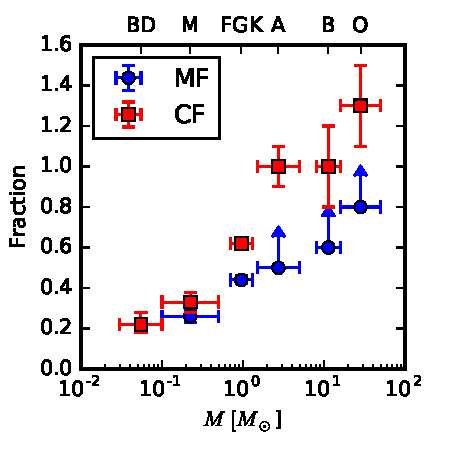
\includegraphics[width=\linewidth]{multiplicity}
\caption[Multiple system fraction versus stellar mass]{
\label{fig:multiplicity}
Multiple system fraction (blue) and companion fraction (red) versus primary star mass for field stars. Horizontal error bars show ranges of mass, and the upper axis shows the spectral type corresponding to that mass, with BD short for brown dwarf. Vertical error bars and limits indicate observational uncertainties. The multiple system fraction is the fraction of stars of that mass that are in multiple systems, while the companion fraction is the mean number of companions per star. The data plotted are taken from Table 1 of \citep{duchene13a}.
}
\end{marginfigure}

First, the binary fraction is a strong function of the mass of the primary star. For O stars it approaches 100\%, while for M and earlier stars it is closer to 20\%. Since the IMF is heavily weighted toward low mass stars (by number), the majority of stars are single -- \citet{lada06a} estimates the single star fraction in the disk today as $60-70\%$. Thus the binary formation mechanism must be strongly mass-dependent. Figure \ref{fig:multiplicity} summarizes this dependence.

Second, the binary period (or separation) distribution is extremely broad and lacks many obvious features \citep{duquennoy91a}. Depending on the stellar mass and the range of periods to which the data are sensitive, this may be fit either by a lognormal in period, or by a flat distribution in $\log P$. The latter is known as \"{O}pik's Law, and it states that there are equal numbers of binaries per logarithmic bin in period (or in semi-major axis). That seems to break down at very large and very small separations, but there is a broad plateau that is close to flat.

For massive stars, there is some evidence for an excess at small separations, indicating an excess of close binaries above what a flat distribution would produce \citep{sana11a}. However it is not entirely clear how much weight to put on this result, since it requires combining data sets gathered in highly different ways (i.e., putting spectroscopic and visual binaries together), and because the selection biases for both data sets are highly complex.

Third, close stellar companions do not appear to be drawn randomly from the IMF. Instead, they are far more likely that a random drawing from the IMF would predict to have masses close to the mass of the primary. In contrast, long-period binaries are consistent with random drawing from the IMF.  We define the mass ratio of a binary consisting of two stars $M_1$ and $M_2$ as $q=M_2/M_1$, where by convention $M_1 > M_2$, so $q$ runs from 0 to 1. Since that the IMF peaks near $0.2$ $\msun$, we would expect random drawing from a sample with primary masses well above $0.2$ $\msun$ to produce many more binaries with small $q$ than large $q$. This is exactly what is seen for distant binaries ($>1000$ day periods), but the opposite trend is seen for closer binaries \citep{mazeh92a, sana11a}.

